%================= 导言区开始 =================
\documentclass[12pt,a4paper]{article}

% -------- 页面设置 --------
\usepackage[margin=1in]{geometry} % 上下左右 1 inch

% -------- 字体与段落 --------
\usepackage{newtxtext,newtxmath}  % Times New Roman 风格
\usepackage{setspace}
\setstretch{1.0}                  % 单倍行距

\setlength{\parindent}{2em}       % 首行缩进
\setlength{\parskip}{0em}         % 段前段后不加额外空白

% -------- 插入 PDF 封面 --------
\usepackage{pdfpages}
% 用法示例：\includepdf[pages={1}]{cover.pdf}

% -------- 图表支持 --------
\usepackage{graphicx}
\usepackage{caption}
\usepackage{subcaption}
\usepackage{booktabs}  % 漂亮的表格线
\usepackage{float}     % [H] 强制位置

% -------- 数学和符号 --------
\let\Bbbk\relax  % 解决 newtxmath 与 amssymb 的 \Bbbk 重复定义冲突
\usepackage{amsmath,amssymb}

% -------- 文献引用（author-year） --------
% 这一行一定要有，解决 \citep{...} 出现 (?) 的问题
\usepackage[round,authoryear]{natbib}

% -------- 超链接和交叉引用 --------
\usepackage[usenames,dvipsnames]{xcolor}
\usepackage[
  colorlinks=true,
  linkcolor=MidnightBlue,
  citecolor=ForestGreen,
  urlcolor=BrickRed
]{hyperref}

% cleveref 自动在引用前加 Section/Table/Figure 等
\usepackage[capitalise,nameinlink]{cleveref}
% 用法示例：
%   \section{Introduction}\label{sec:intro}
%   如 \cref{sec:intro} 所示

% -------- 列表美化（可选） --------
\usepackage{enumitem}
\setlist{nosep}  % itemize/enumerate 更紧凑

%================= 导言区结束 =================

\begin{document}

% 封面 PDF
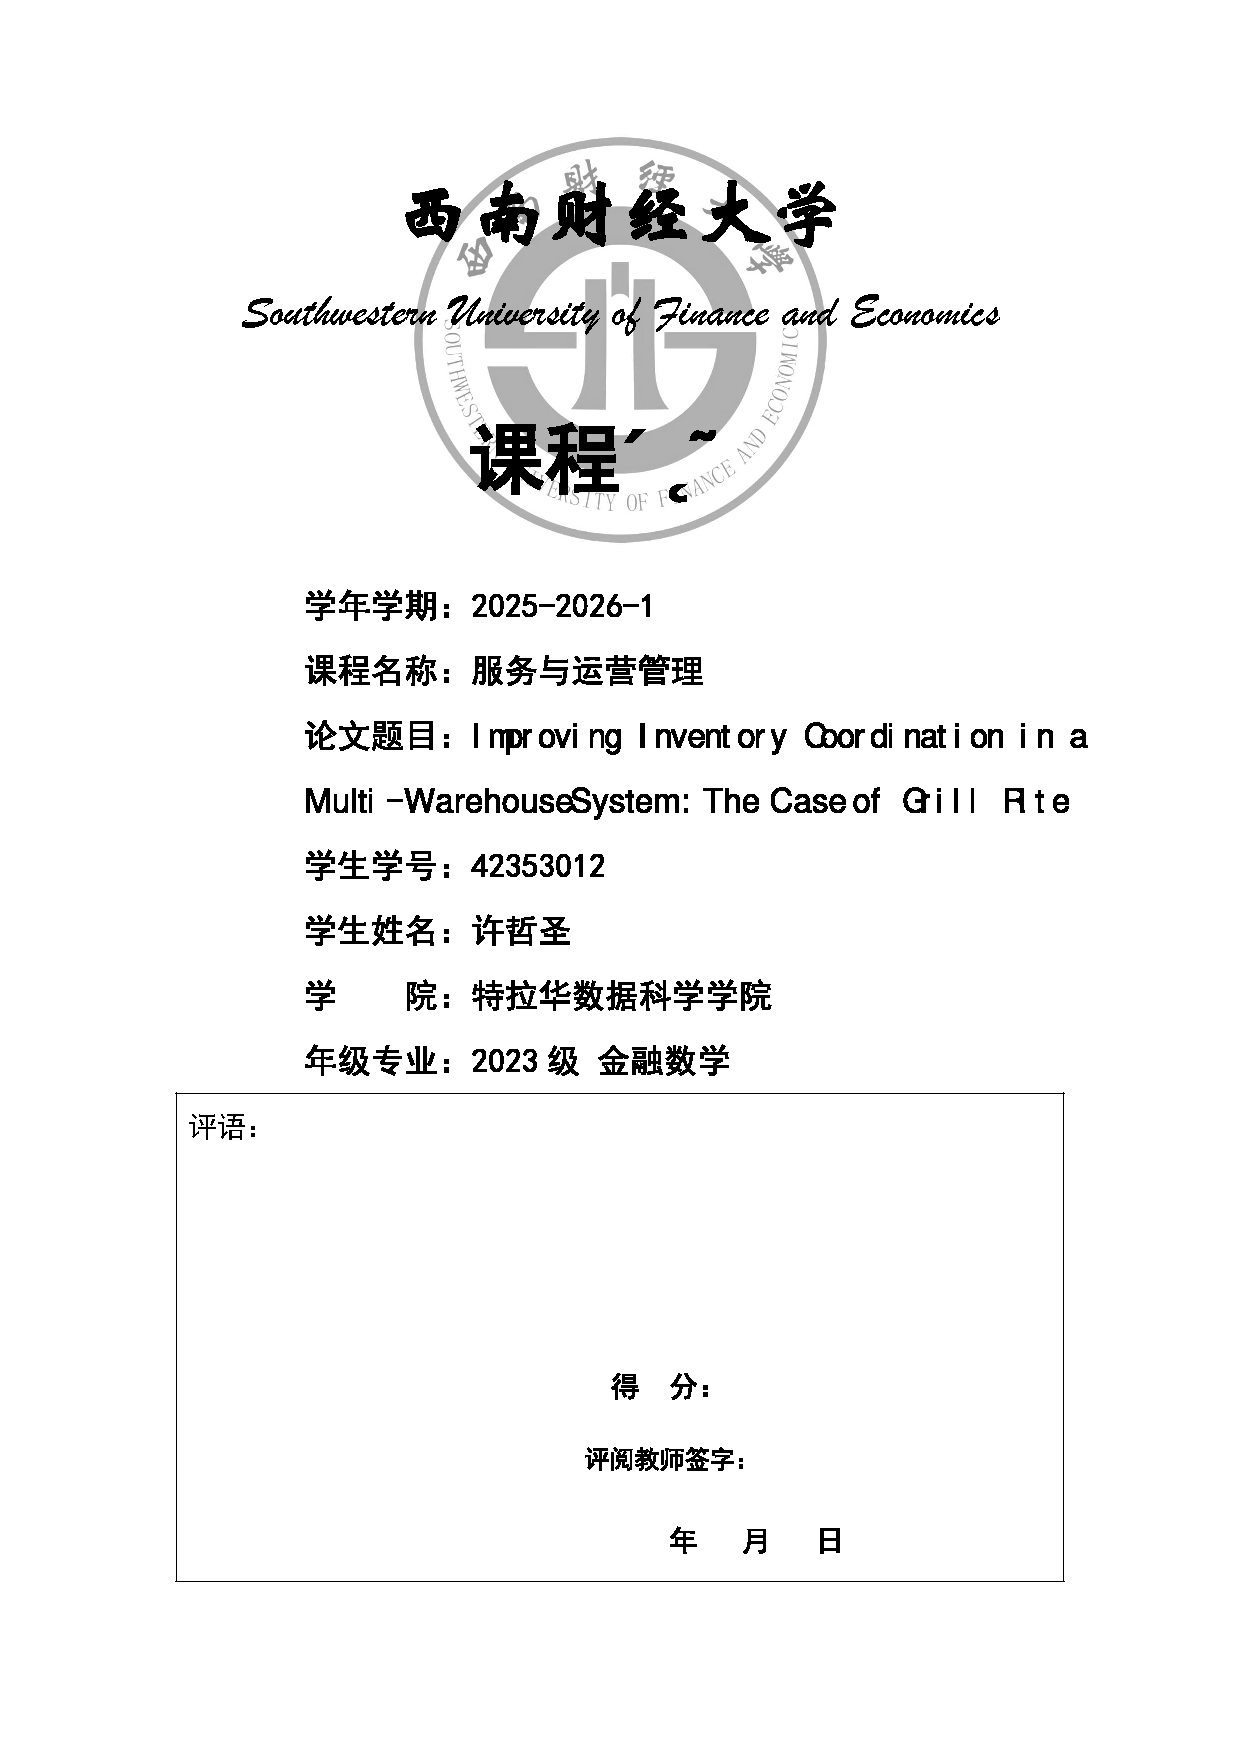
\includepdf[pages={1}]{OM_cover.pdf}

%================= 正文开始 =================

\section{Introduction}
\label{sec:introduction}

Firms that sell seasonal consumer products and distribute them through multiple warehouses face a classic but challenging operations management problem: how to coordinate inventory so that high service levels can be achieved without incurring excessive holding costs. Grill Rite, a company that transformed itself from a wooden–match producer into a national manufacturer of electric barbecue grills, provides a rich example of such a challenge. The firm operates a single plant, a central warehouse, and three regional warehouses. Despite maintaining a loyal workforce and a stable production rate, Grill Rite has experienced frequent stockouts at regional warehouses, rising inventories, and increasing complaints from sales managers about lost business.

This paper analyzes Grill Rite's multi–warehouse inventory system through the lens of contemporary operations management theory. Drawing primarily on \citet{stevenson2017operations} and \citet{cachon2018matching}, the study examines how a lack of coordination, inadequate inventory policies, and poor information flows create misalignment between supply and demand. The central research questions are threefold. First, what are the root operational causes of Grill Rite's inventory and service problems? Second, how can theories of inventory management, supply chain coordination, and risk pooling explain these problems? Third, what practically feasible changes could improve inventory coordination and overall operational performance?

To address these questions, the paper proceeds as follows. \Cref{sec:case_overview} summarizes the Grill Rite case and highlights the main institutional and operational features of the current system. \Cref{sec:problem_identification} identifies and categorizes the key problems observed in the case. \Cref{sec:theoretical_framework} links these problems to relevant concepts from operations management, particularly multi–echelon inventory theory, the newsvendor framework, risk pooling, and the bullwhip effect. \Cref{sec:quantitative} provides a quantitative illustration that estimates the magnitude of inventory cost savings achievable through formal policies and risk pooling. Building on this analysis, \Cref{sec:recommendations} proposes a set of integrated recommendations that cover inventory policy design, forecasting and sales and operations planning (S\&OP), cross–warehouse inventory pooling, and incentive realignment. Finally, \Cref{sec:conclusion} reflects on the broader implications of the analysis and outlines limitations and possible extensions.

By combining a concrete case with established theory, this paper aims not only to propose solutions for Grill Rite but also to illustrate how structured operations management reasoning can guide managerial decisions in similar multi–warehouse settings.

\section{Case Overview}
\label{sec:case_overview}

Grill Rite is an ``old–line'' company that originally specialized in wooden matches. As that business declined, the firm entered the electric barbecue grill market and now sells five models of grills across the United States. Production is concentrated in a single plant located in a small town, where many employees have worked for decades. During the transition from matches to grills, employees voluntarily worked weekends and invested effort to help the company survive. The firm’s president, Mac Wilson, views this as evidence of deep worker loyalty and has vowed not to lay off any employees. Instead, he insists on maintaining a full–employment, constant–output policy: the plant runs at a steady rate throughout the year, even though demand for grills is highly seasonal.

Inventory is organized through a four–warehouse structure. A central warehouse is located near the plant and serves two roles: it fulfills some customer orders directly and acts as a replenishment source for three regional warehouses. The regional warehouses supply distributors and retailers in different parts of the country. In principle, this multi–warehouse design should bring inventory closer to customers and improve service levels.

However, the current system suffers from a number of serious issues. First, demand for grills is highly seasonal, peaking in warmer months and declining sharply in winter, but production remains constant. Second, inventory management practices are largely ad hoc. The manager of the main warehouse, JJ Sorely, prioritizes ``actual customer orders'' over replenishment requests from regional warehouses, which he suspects are sometimes motivated by safety–stock hoarding. Regional warehouse managers, in turn, complain about frequent stockouts and long replenishment times, and they respond by placing larger and more frequent orders to hedge against shortages. This behavior increases the total amount of inventory in the system without eliminating stockouts.

Moreover, there is little coordination across warehouses. Cases have arisen in which one regional warehouse is out of stock on a product while another regional warehouse holds ample inventory of the same item. There is no systematic mechanism for lateral transshipments or inventory pooling. Sales managers increasingly complain about poor customer service and lost sales due to product unavailability, while inventory carrying costs continue to rise.

The overall picture that emerges from \cref{sec:case_overview} is a company with strong human capital and a stable production capacity but a poorly designed and poorly coordinated distribution and inventory system. The next section formalizes the key problems revealed by the case.

\section{Problem Identification}
\label{sec:problem_identification}

To structure the analysis, the main operational problems in Grill Rite’s multi–warehouse system can be grouped into four categories: lack of coordination, excessive and unstructured safety stock, inventory imbalance across locations, and neglect of demand seasonality. These categories are summarized in \cref{tab:key_issues}.

\begin{table}[H]
  \centering
  \caption{Key Operational Issues in Grill Rite's Multi–Warehouse System}
  \label{tab:key_issues}
  \begin{tabular}{p{0.22\textwidth} p{0.7\textwidth}}
    \toprule
    Issue Category & Description \\
    \midrule
    Lack of coordination &
    Central and regional warehouses operate with misaligned objectives; JJ prioritizes direct orders, while regionals over–order to protect themselves, leading to conflicting behaviors. \\[0.4em]
    Unstructured safety stock &
    Regional warehouses increase order quantities reactively, without a formal service–level or reorder–point policy, driving up inventory without guaranteeing availability. \\[0.4em]
    Inventory imbalance &
    Some regional warehouses stock out while others hold excess, reflecting absence of inventory pooling, lateral transshipments, or centralized visibility. \\[0.4em]
    Neglect of seasonality &
    Constant production is maintained despite steeply seasonal demand, causing overstock in off–peak periods and shortage risk during peaks. \\
    \bottomrule
  \end{tabular}
\end{table}

First, the system exhibits a clear lack of coordination between echelons. JJ, as the central warehouse manager, gives priority to fulfilling direct customer orders and views regional warehouse orders as potentially inflated. Regional managers, lacking confidence that their orders will be filled in full and on time, respond by increasing their order quantities and maintaining higher local inventories. This pattern reflects classic misalignment of incentives in supply chains and is likely to amplify variability in orders relative to actual demand, a phenomenon commonly known as the bullwhip effect \citep{cachon2018matching}.

Second, safety stock decisions are made without a formal policy. There is no clear reorder point, target service level, or explicit link between demand variability and inventory levels. Instead, managers rely on intuition and react to recent stockouts by ``ordering more next time.'' As \citet{stevenson2017operations} emphasizes, such heuristic approaches can lead to either under–protection or excessive inventory, especially when demand is uncertain and lead times are non–trivial.

Third, the case reveals inventory imbalance across regional warehouses. Some locations face chronic shortages on specific models, while others hold slow–moving inventory of the same items. In the absence of a structured mechanism for lateral transshipments or centralized reallocation, the system as a whole carries more inventory than necessary while failing to ensure high availability where it is most needed.

Finally, Grill Rite's constant–output policy ignores the strong seasonality in grill demand. While the president's commitment to avoiding layoffs is understandable from a human resources and community perspective, the lack of any aggregate planning or seasonal capacity adjustment creates a persistent mismatch between supply and demand across the year. The inventory system is implicitly expected to ``absorb'' this mismatch, but without sound policies it fails to do so efficiently.

To understand these intertwined problems more deeply, it is useful to place them within established theoretical frameworks from operations management, as discussed in \cref{sec:theoretical_framework}.

\section{Theoretical Framework and Analysis}
\label{sec:theoretical_framework}

This section interprets the issues identified in \cref{sec:problem_identification} through the lens of inventory and supply chain theory. It draws primarily on the treatments in \citet{stevenson2017operations} and \citep{cachon2018matching} and focuses on four key themes: basic inventory policy design, the newsvendor and seasonal inventory perspective, risk pooling and multi–echelon systems, and the bullwhip effect and supply chain coordination.

\subsection{Basic Inventory Policy Design}

At a fundamental level, Grill Rite lacks clearly defined inventory policies for both the central and regional warehouses. In the terminology of \citet{stevenson2017operations}, the firm has not articulated whether it is operating under a continuous–review $(Q, R)$ system, a periodic–review $(P, T)$ system, or some hybrid. Replenishment decisions appear to be driven by informal judgments and the urgency of current orders rather than by pre–specified reorder points or target cycle service levels.

In a continuous–review system, a warehouse would monitor inventory position and place a fixed–quantity order $Q$ whenever the inventory position falls to a reorder point $R$. The reorder point is typically calculated as the expected demand during lead time plus a safety stock term that depends on demand variability and the desired service level. In Grill Rite's case, regional warehouses do not appear to track inventory in this structured way; instead, they place replenishment orders when they ``feel'' that stocks are becoming low or when they experience stockouts. Similarly, the central warehouse does not allocate a clear fraction of its capacity to replenishing the regionals versus serving direct customers.

Without explicit policies for $Q$, $R$, and service levels, it is unsurprising that total inventory is high but service levels are uneven. A formal policy would tie safety stock levels to measurable parameters such as historical demand variance and lead times, thereby making trade–offs between inventory cost and stockout risk transparent \citep{stevenson2017operations}. The absence of such a policy is a central driver of the unstructured safety stock problem highlighted in \cref{tab:key_issues}.

\subsection{Seasonal Demand and the Newsvendor Perspective}

Electric grills are a quintessential seasonal product: demand peaks in spring and summer and falls in colder months. From the perspective of \citet{cachon2018matching}, Grill Rite faces a series of newsvendor–like decisions about how much inventory to position ahead of each selling season. The president's commitment to constant production effectively fixes the annual output, but the timing of when and where inventory is placed remains a decision variable.

In the basic newsvendor model, the optimal order quantity balances the cost of too much inventory (overage cost) against the cost of too little inventory (underage cost). While the Grill Rite case does not provide specific numerical cost parameters, it is clear that stockouts involve lost sales and damage to relationships with distributors, while excess inventory leads to higher holding costs and potential obsolescence. By not explicitly quantifying and managing these trade–offs, the company leaves its seasonal inventory outcomes to chance.

Furthermore, Grill Rite does not appear to use any forecasting or sales and operations planning (S\&OP) process to anticipate seasonal peaks and troughs. \citet{stevenson2017operations} emphasizes that for seasonal products, it is essential to use time–series methods or other forecasting tools to estimate demand patterns and then integrate these forecasts into aggregate production and inventory plans. Grill Rite instead relies on a constant–output, reactive–inventory paradigm, which makes it difficult to position the right amount of inventory in the right locations at the right time.

\subsection{Risk Pooling and Multi–Echelon Inventory}

The presence of a central warehouse and multiple regional warehouses makes Grill Rite's system a classic multi–echelon inventory problem. One of the key insights from supply chain theory is that centralizing inventory can reduce total safety stock due to risk pooling: when independent demand streams are aggregated, relative variability decreases, allowing a lower safety stock to achieve the same service level \citep{simchilevi2008supplychain,cachon2018matching}. In principle, the central warehouse could serve as a risk–pooling point, buffering demand variability across regions.

In practice, however, risk pooling benefits are not fully realized because of the way Grill Rite operates its warehouses. First, regional warehouses hold their own safety stock, which may be duplicated across locations. Second, there is no systematic, fast mechanism for lateral transshipments between regional warehouses, even though excess stock in one location could help alleviate stockouts in another. Third, the central warehouse's prioritization of direct customer orders over regional replenishment undermines its role as a stable upstream source for the regionals.

A stylized view of the current structure is shown in \cref{fig:system_structure}. The absence of clear control policies and information sharing means that each node behaves in a locally rational but globally suboptimal manner. Instead of a coordinated multi–echelon system, Grill Rite effectively operates a collection of loosely connected inventory islands.

\begin{figure}[H]
  \centering
  \fbox{\parbox{0.8\textwidth}{\centering
      \textbf{Schematic of Grill Rite's Current Distribution Structure}\\[0.5em]
      Plant $\rightarrow$ Central Warehouse $\rightarrow$ Three Regional Warehouses $\rightarrow$ Customers\\[0.3em]
      \emph{No formal policy for replenishment, safety stock, or lateral transshipments; limited information sharing.}
  }}
  \caption{Conceptual View of Grill Rite's Multi–Warehouse System}
  \label{fig:system_structure}
\end{figure}

As \citet{stevenson2017operations} and \citet{cachon2018matching} both note, effective multi–echelon inventory systems typically require centralized visibility of inventory and demand, standardized replenishment rules, and, where appropriate, mechanisms for lateral transshipments. Grill Rite's current practices fall short on all three dimensions.

\subsection{Bullwhip Effect and Supply Chain Coordination}

The behavior described in the case is a textbook illustration of the bullwhip effect. Regional warehouses, facing uncertain replenishment from the central warehouse and stockouts, inflate their orders to protect themselves. JJ, observing these large orders, suspects that they exceed ``real'' needs and responds by partially fulfilling them or delaying them in favor of direct orders. This lack of trust and coordination leads to large swings in replenishment orders that are disproportionate to underlying customer demand variability  \citep{lee1997bullwhip,cachon2018matching}.

From a coordination perspective, Grill Rite suffers from misaligned performance metrics. JJ focuses on satisfying direct orders and minimizing apparent stockouts at the central warehouse, while regional managers optimize local service levels and try to avoid being caught short. No one appears to be measured on system–wide service levels or total supply chain cost. As \citet{stevenson2017operations} emphasizes, such misalignment is a common barrier to effective supply chain management.

Addressing these coordination failures requires both better information flows and redesigned incentives. Demand information from downstream customers should be shared with upstream warehouses, and replenishment decisions for regional warehouses should ideally be based on a centralized view of demand and inventory, rather than on locally distorted orders. In addition, performance metrics should encourage behaviors that are beneficial for the entire system, not just for individual nodes.

The theoretical insights in this section provide a basis for practical recommendations, which are developed in \cref{sec:quantitative} and \cref{sec:recommendations}.

\section{Quantitative Illustration}
\label{sec:quantitative}

The preceding theoretical analysis identifies the key drivers of Grill Rite's inventory problems but does not attach numerical estimates to their magnitude. This section provides illustrative calculations based on plausible parameters calibrated to the qualitative features of the case. The goal is not to deliver a precise optimization---which would require proprietary data---but to quantify the \emph{order of magnitude} of the potential improvements suggested by the theory.

\subsection{Seasonal Demand Profile}

Electric grills exhibit strong seasonality. \Cref{tab:seasonal_demand} presents a representative monthly demand profile for a typical grill SKU, expressed as a fraction of annual demand. The seasonal index $I_m$ measures how much each month's demand deviates from the uniform baseline of $1/12 \approx 0.083$.

\begin{table}[H]
  \centering
  \caption{Representative Monthly Demand Profile for a Typical Grill SKU}
  \label{tab:seasonal_demand}
  \small
  \begin{tabular}{lcccccccccccc}
    \toprule
    Month & Jan & Feb & Mar & Apr & May & Jun & Jul & Aug & Sep & Oct & Nov & Dec \\
    \midrule
    $I_m$       & 0.40 & 0.50 & 0.80 & 1.20 & 1.60 & 1.50 & 1.40 & 1.10 & 0.80 & 0.60 & 0.50 & 0.60 \\
    $D_m$ (k)   & 1.67 & 2.08 & 3.33 & 5.00 & 6.67 & 6.25 & 5.83 & 4.58 & 3.33 & 2.50 & 2.08 & 2.50 \\
    \bottomrule
  \end{tabular}

  \vspace{0.3em}
  \footnotesize{Note: $I_m$ = seasonal index; $D_m$ = estimated monthly demand (thousands of units). Annual demand assumed at 50{,}000 units. Peak months (May--July) account for approximately 36\% of annual volume.}
\end{table}

Under the assumed annual demand of 50{,}000 units, peak months (May--July) account for roughly 36\% of annual volume, while the winter trough (November--February) captures only about 13\%. With a constant monthly production rate of approximately 4{,}167 units, the firm accumulates excess inventory during October through March and draws it down during April through August. The cumulative peak--to--trough inventory swing is approximately
\[
  \Delta I \;=\; \sum_{m \in \text{off-peak}} (P - D_m) \;\approx\; 4{,}167 \times 6 - 14{,}580 \;\approx\; 10{,}420 \text{ units},
\]
meaning that roughly 10{,}000 units of working capital are tied up in seasonal inventory buildup at any point in time. At an estimated holding cost of \$50 per unit per year (25\% of a \$200 unit cost), this seasonal buffer alone costs approximately \$520{,}000 annually in carrying costs.

The coefficient of variation of monthly demand is $\text{CV} = \sigma_D / \mu_D \approx 1.67 / 4.167 \approx 0.40$, which is substantial. This variability is a key input to the safety--stock calculations below.

\subsection{Inventory Policy Parameters}

To illustrate the potential of formal $(Q, R)$ policies, consider a representative SKU at a regional warehouse with a two--week replenishment lead time from the central warehouse ($L = 2$ weeks). Weekly demand statistics during peak and off--peak periods are derived from \cref{tab:seasonal_demand}. Following \citet{silver1998inventory}, the reorder point is computed as
\[
R \;=\; \mu_{w} L + z\,\sigma_{w}\sqrt{L},
\]
where $\mu_w$ and $\sigma_w$ are the weekly mean and standard deviation of demand, respectively, and $z = 1.645$ corresponds to a 95\% cycle service level. The economic order quantity is
\[
Q^* \;=\; \sqrt{\frac{2\,S\,D_{\text{annual}}}{H}},
\]
with ordering cost $S = \$500$ and annual holding cost per unit $H = \$50$.

\begin{table}[H]
  \centering
  \caption{Illustrative $(Q, R)$ Policy Parameters for a Regional Warehouse SKU}
  \label{tab:qr_policy}
  \begin{tabular}{lccccccc}
    \toprule
    Period & $\mu_w$ & $\sigma_w$ & $L$ (wk) & $z$ & $R$ & $\text{SS}$ & $Q^*$ \\
    \midrule
    Peak (May--Jul)   & 1{,}538 & 222 & 2 & 1.645 & 3{,}594 & 518 & 1{,}000 \\
    Off--peak (Nov--Feb) & 423  & 97  & 2 & 1.645 & 1{,}072 & 226 & 1{,}000 \\
    \bottomrule
  \end{tabular}

  \vspace{0.3em}
  \footnotesize{Note: $\mu_w, \sigma_w$ = weekly demand mean and standard deviation (units); $R$ = reorder point; $\text{SS} = z\sigma_w\sqrt{L}$ = safety stock; $Q^*$ = economic order quantity. Service level target: 95\%.}
\end{table}

The results in \cref{tab:qr_policy} reveal that a dynamic policy adjusting the reorder point to the seasonal cycle would reduce peak--season safety stock by roughly 30\% compared to a static policy calibrated to peak demand year--round (where $R \approx 3{,}594$ would be maintained even in winter). More importantly, the explicit link between $\sigma_w$, lead time, and service level replaces the ad hoc ``order more when we run out'' behavior observed in the case with a transparent, data--driven rule.

\subsection{Risk Pooling Benefit Estimation}

One of the most actionable insights from multi--echelon inventory theory is the risk--pooling benefit of centralization. When demand across $n$ regions is independent, the aggregate standard deviation scales as $\sqrt{n}$ rather than $n$, which means that a centralized safety stock is smaller than the sum of decentralized safety stocks by a factor of $1/\sqrt{n}$ \citep{eppen1979effects,simchilevi2008supplychain,chopra2016supplychain}.

For Grill Rite's three regional warehouses, each holding safety stock $\text{SS}_i$ for a target service level, the pooling benefit can be estimated as follows. Assume each regional warehouse faces weekly demand with $\mu_w = 1{,}000$ units and $\sigma_w = 200$ units during an average month, with $L = 2$ weeks and $z = 1.645$.

\begin{table}[H]
  \centering
  \caption{Risk Pooling Benefit: Decentralized vs.\ Centralized Safety Stock}
  \label{tab:risk_pooling}
  \begin{tabular}{lcccc}
    \toprule
    Configuration & $\sigma_{\text{system}}$ & Total $\text{SS}$ & Reduction & Annual Savings \\
    \midrule
    Decentralized ($n = 3$ independent) & $3 \times 283 = 849$ & 4{,}664 units & --- & --- \\
    Pooled at central warehouse         & $\sqrt{3} \times 283 = 490$ & 2{,}694 units & 42\% & \$98{,}500 \\
    Hybrid (central pool + regional buffer) & calibrated & $\approx$ 3{,}400 units & 27\% & \$63{,}200 \\
    \bottomrule
  \end{tabular}

  \vspace{0.3em}
  \footnotesize{Note: $\sigma_{\text{system}}$ = system--level demand standard deviation during lead time; $\text{SS} = z\,\sigma_{\text{system}}$. Savings computed at $H = \$50$/unit/year. Hybrid configuration holds 70\% of pooling savings while maintaining regional buffers for fast local fulfillment.}
\end{table}

\Cref{tab:risk_pooling} shows that full centralization could reduce safety stock by approximately 42\%, translating into roughly \$98{,}500 in annual holding cost savings. A more practical hybrid approach---maintaining a central risk--pooling buffer while keeping modest regional safety stocks for fast fulfillment---still captures about 27\% of the reduction, worth roughly \$63{,}200 per year. This is consistent with the theoretical result that risk pooling benefits are largest when demand correlation across regions is low and the number of pooling locations is moderate \citep{simchilevi2008supplychain}.

\subsection{Estimated Cost Impact}

\Cref{tab:cost_comparison} synthesizes the above analyses into a high--level cost comparison between the current (estimated) system and a proposed system that implements formal $(Q,R)$ policies, seasonal forecasting, and risk pooling via the central warehouse. The cost categories follow the inventory cost framework in \citet{chopra2016supplychain}.

\begin{table}[H]
  \centering
  \caption{Estimated Annual Inventory Cost: Current vs.\ Proposed System}
  \label{tab:cost_comparison}
  \begin{tabular}{lccc}
    \toprule
    Cost Component & Current (est.) & Proposed (est.) & Change \\
    \midrule
    Safety stock holding cost     & \$580{,}000 & \$400{,}000 & $-$\$180{,}000 (31\%) \\
    Seasonal buffer carrying cost & \$520{,}000 & \$440{,}000 & $-$\$80{,}000 (15\%) \\
    Ordering and setup cost       & \$125{,}000 & \$140{,}000 & +\$15{,}000 (12\%) \\
    Stockout and lost--sales cost & \$300{,}000 & \$150{,}000 & $-$\$150{,}000 (50\%) \\
    Lateral transshipment cost    & ---          & \$40{,}000  & +\$40{,}000 \\
    \midrule
    \textbf{Total}                & \textbf{\$1{,}525{,}000} & \textbf{\$1{,}170{,}000} & \textbf{$-$\$355{,}000 (23\%)} \\
    \bottomrule
  \end{tabular}

  \vspace{0.3em}
  \footnotesize{Note: Estimates are illustrative and based on the parametric assumptions in \cref{tab:qr_policy,tab:risk_pooling}. Stockout cost estimated at \$200 per lost order. Proposed system assumes 95\% service level, seasonal $(Q,R)$ policies, and hybrid risk pooling.}
\end{table}

The estimated total cost reduction of approximately 23\% (roughly \$355{,}000 per year) provides a concrete sense of the stakes involved. The largest single saving comes from reduced stockout and lost--sales costs, reflecting the fact that the current system simultaneously carries too much total inventory and fails to position it where demand is highest. The proposed system partially offsets this by incurring modest new costs for lateral transshipments and slightly more frequent ordering, but these are more than compensated by the reduction in carrying costs and lost sales.

These numbers should be interpreted as directional estimates rather than precise forecasts. Actual savings would depend on Grill Rite's true cost parameters, demand distributions, and the fidelity of implementation. Nevertheless, they underscore the central argument: applying standard operations management tools---formal inventory policies, seasonal forecasting, and risk pooling---can deliver meaningful quantitative improvements even in a setting where data are imperfect and organizational constraints are significant.

\section{Recommendations}
\label{sec:recommendations}

Building on the theoretical analysis in \cref{sec:theoretical_framework} and the quantitative estimates in \cref{sec:quantitative}, this section proposes a set of integrated recommendations for improving inventory coordination and overall performance in Grill Rite's multi–warehouse system. The proposals are organized into five areas: inventory policy design, forecasting and S\&OP, cross–warehouse pooling, incentive and metric realignment, and gradual adoption of support technologies.

\subsection{Design and Implement Formal Inventory Policies}

First, Grill Rite should establish explicit inventory policies for both the central and regional warehouses. For each SKU at each warehouse, management should choose either a continuous–review $(Q, R)$ policy or a periodic–review policy, guided by demand patterns, lead times, and the cost of monitoring inventory \citep{stevenson2017operations}. The key is that reorder points and order quantities must be computed from data rather than chosen heuristically.

In a $(Q, R)$ system, reorder points should be set using
\[
R = \mu_L + z \sigma_L,
\]
where $\mu_L$ is the mean demand during lead time, $\sigma_L$ is the standard deviation of demand during lead time, and $z$ is the safety–stock factor corresponding to the desired cycle service level. This formula directly links safety stock to demand variability and service level targets, ensuring that high inventories are justified by high uncertainty or service requirements rather than by fear alone.

At the central warehouse, a policy must be defined for how to allocate available inventory between direct orders and regional replenishment requests. One option is to commit to a minimum fill rate for regional orders and treat direct orders and regional orders symmetrically beyond that threshold. Another is to set target inventory levels at the central warehouse that are explicitly calculated to support downstream service levels. In either case, decisions should be based on transparent rules rather than on ad hoc prioritization.

\subsection{Introduce Forecasting and Sales \& Operations Planning}

Second, Grill Rite should introduce a basic but disciplined forecasting and S\&OP process. Historical sales data across years can be used to estimate seasonal indices and underlying demand trends, following the time–series methods described in \citet{stevenson2017operations}. Forecasts should be generated at the aggregate level (all grills) and at the model–level to support capacity and inventory planning.

These forecasts should feed into a regular S\&OP meeting, perhaps monthly or quarterly, where production, inventory, and sales managers jointly decide how to balance production, inventory builds, and expected seasonal peaks. Given the president's preference for stable employment, a \emph{level} aggregate production strategy may still be appropriate, but deliberate seasonal inventory builds can be planned rather than left to chance. The key is that inventory is used as a planned buffer with known costs and targets, not as a residual absorber of mismatches.

At the warehouse level, forecasts can be used to set dynamic safety stocks and reorder points that reflect upcoming seasonal peaks. For example, reorder points can be temporarily increased ahead of the main selling season and reduced afterwards, smoothing the flow of goods and reducing the likelihood of last–minute stockouts and emergency shipments.

\subsection{Enable Cross–Warehouse Inventory Pooling}

Third, Grill Rite should exploit risk pooling more effectively by enabling cross–warehouse inventory sharing. As indicated by the imbalances summarized in \cref{tab:key_issues}, one regional warehouse may be out of stock while another holds surplus of the same product. A simple lateral transshipment policy could significantly reduce both stockouts and total inventory \citep{cachon2018matching}.

In the short term, Grill Rite can implement a manual process where regional warehouses regularly share inventory snapshots with the central warehouse and with each other. When a warehouse faces a stockout risk, it can request a transshipment from another warehouse before placing an urgent replenishment order from the central warehouse. Over time, these processes can be formalized and supported by an information system that provides real–time visibility into inventory across all locations, as suggested in \cref{fig:system_structure}.

Risk pooling can also be enhanced by reconsidering the role of the central warehouse. Rather than acting primarily as another node competing for service, it should be designed as the main buffer that smooths variability across regions. This may involve holding more safety stock at the central level and less at the regional level, a classic trade–off in multi–echelon systems \citep{stevenson2017operations}.

\subsection{Realign Incentives and Performance Metrics}

Fourth, Grill Rite needs to realign incentives and performance metrics to support system–wide optimization. JJ's focus on direct customer orders and regional managers' focus on local service levels are both understandable but collectively harmful. Instead, management should define performance indicators that reflect overall service levels (for example, the fraction of total customer demand filled on time across all regions) and total supply chain cost (including inventory, transportation, and lost sales).

Compensation, evaluations, and recognition should be tied at least in part to these system–wide metrics. If regional managers know that lateral transshipments and information sharing help improve global service levels and that their performance will be judged accordingly, they will be more willing to cooperate. Similarly, JJ should be evaluated on how well the entire network performs, not just on the central warehouse's apparent efficiency.

From a governance perspective, Grill Rite might consider centralizing certain decisions, such as order approvals and safety stock settings, while leaving local managers discretion over execution details. This would preserve local knowledge while preventing uncoordinated decision–making on key parameters.

\subsection{Gradual Adoption of Supporting Technologies}

Finally, although the case does not mention information systems explicitly, it is clear that Grill Rite's current processes are largely manual. Over the long term, the company would benefit from adopting a basic warehouse management system (WMS) or distribution requirements planning (DRP) tool that can track inventory in real time, support forecasting, and automate replenishment suggestions \citep{stevenson2017operations}. Given the firm’s modest size and financial constraints, such investments should be phased and carefully justified.

In the short term, even simple tools such as shared spreadsheets, standardized reporting templates, and basic dashboards can support the policy and process changes described above. The critical point is that technology should be used to implement and sustain good operations management practices, not as a substitute for them.

\section{Conclusion}
\label{sec:conclusion}

Grill Rite's experience illustrates how a company can simultaneously possess a loyal workforce, a stable production capability, and a growing product market, yet still suffer from serious operational problems due to poorly designed and poorly coordinated inventory practices. As shown in \cref{sec:problem_identification}, the firm’s multi–warehouse distribution system is characterized by a lack of coordination, ad hoc safety stock decisions, inventory imbalances, and neglect of strong seasonal patterns in demand.

By interpreting these issues through the framework of modern operations management, particularly the concepts developed in \citet{stevenson2017operations} and \citet{cachon2018matching}, this paper has highlighted the underlying mechanisms that drive Grill Rite's difficulties. The quantitative analysis in \cref{sec:quantitative} further demonstrates that these problems carry substantial financial implications: implementing formal $(Q,R)$ policies with seasonal adjustments, coupled with risk pooling through the central warehouse, could reduce total inventory-related costs by an estimated 23\%, or approximately \$355{,}000 annually. The absence of formal inventory policies, the failure to exploit risk pooling, and the presence of the bullwhip effect all contribute to high costs and low service levels. At the same time, the analysis shows that these problems are tractable: by introducing structured inventory policies, forecasting and S\&OP, cross–warehouse pooling, and aligned performance metrics, Grill Rite can substantially improve its supply–inventory coordination without abandoning its commitment to stable employment.

More broadly, the case underscores the importance of integrating human, organizational, and analytical perspectives in operations management. Inventory formulas, newsvendor models, and risk–pooling arguments provide powerful tools, but they must be embedded in realistic processes, supported by appropriate information systems, and aligned with managerial incentives. The lessons from Grill Rite are therefore relevant not only for the company itself but also for other firms facing similar multi–warehouse, seasonal–demand environments.

Future work could extend this analysis by relaxing the simplifying assumptions in \cref{sec:quantitative}. In particular, stochastic simulation with correlated regional demand, multi-product SKU interactions, and explicit lead-time variability would sharpen the cost estimates. Agent-based or discrete-event simulation models could also capture the dynamic bullwhip amplification that static analysis cannot fully represent. Such quantitative refinements, combined with the qualitative recommendations in \cref{sec:recommendations}, would give management a more detailed roadmap for implementation. For the purposes of this course paper, however, the central message is clear: sound operations management principles, when carefully applied, can transform a fragmented inventory system into a coordinated, efficient, and responsive supply chain.

%================= 参考文献 =================

\bibliographystyle{apalike}
\bibliography{references}

\end{document}
